\documentclass[12pt]{article}
%Gummi|065|=)
\usepackage[utf8]{inputenc}
\usepackage{graphicx}
\title{\textbf{Welcome to Gummi 0.6.5}}
\author{Maj Smerkol  - 63120278\\
Študijsko leto 2014/15 \\
Spletno programiranje}
\date{\today}
\begin{document}

\maketitle

\section{Spletna aplikacija}
ToDo List 
\includegraphics[scale=0.1]{todo_logo.png} je spletna aplikacija, namenjena vzpodbujanju uporabnika k izpolnjevanju svojih obveznosti. To aplikacija doseže tako, da uporabniku pomaga pri pripravi dnevnega plana in ga opozarja na pomemebna opravila v bližnji prihodnosti.

Uporabnik v aplikacijo doda opravila. Vsakemu opravilu lahko nastavi oznako (ime), rok za dokončanje, pomembnost (številčna vrednost od 1 do 5) in opis, v katerem poda podrobnosti o opravilu. Names opisa je, da uporabnik lažje prikliče v spomin opravilo in ne podrobnem razčlenjevanju opravila. 

\section{Ciljna publika}
Ciljna publika aplikacije ToDo List so srednje zahtevni uporabniki, ki želijo predvsem dostop do svojih zapiskov prek interneta in opozarjanje, da opravila dejansko opravijo. V tej skupini sem prepoznal predvsem študente in dijake, saj poslovni uporabniki potrenujejo več.

\newpage
\section{Organizacija spletišča}
Aplikacija je organizirana naključno, vendar zelo preprosto, da se uporabnik ne izgubi na strani.

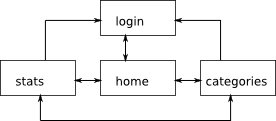
\includegraphics[scale=1.4]{sitemap01.png}

S strani \texttt{login} se uporabnik vpiše na stran ali pa se registrari, če še nima uporabniškega imena. 

Ko to stori, pride na stran \texttt{home}, kjer vidi plan za današnji dan in vse ostale naloge, ki jih mora opraviti. Tukaj lahko tudi doda nova opravila, spreminja obstoječa in jih izbriše.

Na strani \texttt{categories} vidi vsa opravila, urejena v kategorije. Tukaj lahko opravila spreminja in jih briše.

Na strani \texttt{stats} lahko uporabnik vidi statistične podatke o svoji uspešnosti pri opravljanju nalog. Aplikacija zanj izriše graf števila opravljenih nalog v odvisnosti od časa (na dan natančno). Tako lahko uporabnik za vsak dan vidi, koliko koristnega dela je opravil.

Izpisani so tudi nekateri drugi podatki. Ker je ciljna publika mlada, se izpišejo tudi uporabnikovi dosežki, ki se beležijo sproti. To naj bi uporabnika motiviralo k delu.

Iz menijske vrstice lahko z vseh strani, razen \texttt{login}, dostopa do vseh ostalih strani. Tako lahko do vseh delov strani uporabnik dostopa do vseh drugih.

\newpage
\section{Struktura spletišča}
Pri oblikovanju strukture sem se zgledoval po strani Google Keep, ki je po funkcijonalnostih prav tako podobna. 

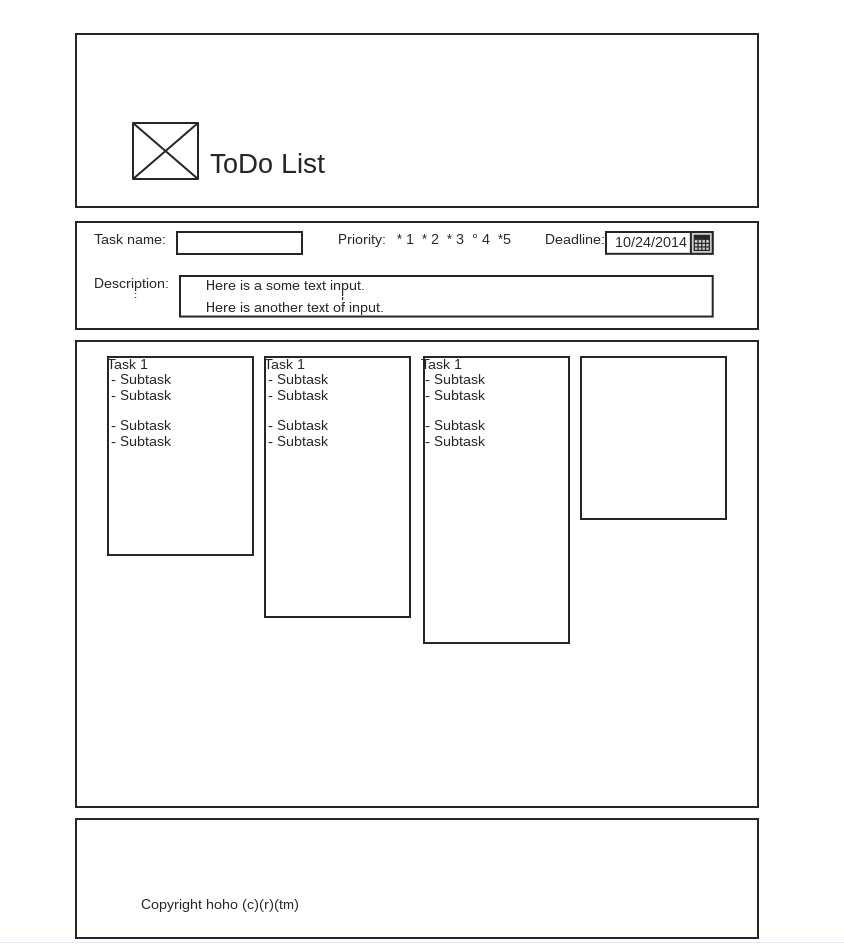
\includegraphics[scale=0.4]{wireframe_main.png}

Držal sem se kalsične strukture z glavo, telesom in nogo. V glavi je logo in menijska vrstica, v telesu je vsa vsebina, v nogi pa kontaktne informacije.

\newpage
\section{Oblikovanje}
Vse strani so oblikovane po enakem principu. Glava in noga sta povsod enaki, saj to pripomore k enotnosti izgleda strani. Na vseh straneh spletišča se pojavljajo podobni elementi: telo je razdeljeno z naslovi, ki razlagajo funkcionalnost dela strani, pod njimi pa so elementi. Da se bolje loči dele strani, so naslovi napisani na kontrastnem ozadju. Elementi vsebine so povsod v poljih temnnejše barve, da se lahko posamezne elemente loči, kljub temu pa zaradi vmeščenosti med naslove delujejo kot celota.

Ciljna publika je mlada, vendar pa je ta aplikacija namenjena produktivnosti in ne zabavi, zato sem se odločil za ne preveč svetlo barvno shemo. Modra barva, na kateri celotna shema temelji, uporabnika pomirja. Celotna shema je precej hladna, s čimer nakazuje na resen namen aplikacije. 

\vspace{15pt}


\includegraphics[scale=1.5]{barvna_shema.png}



\end{document}
